
% Decision tree
% Author: Stefan Kottwitz
% https://www.packtpub.com/hardware-and-creative/latex-cookbook
\documentclass[border=10pt]{standalone}
\usepackage{tikz}
\tikzset{
	treenode/.style = {shape=rectangle, rounded corners,
		draw, align=center,
		top color=white, bottom color=blue!20},
	root/.style     = {treenode, font=\Large, bottom color=red!30},
	env/.style      = {treenode, font=\ttfamily\normalsize},
	dummy/.style    = {circle,draw}
%	action/.style   = {rectangle,draw}
}
\begin{document}
	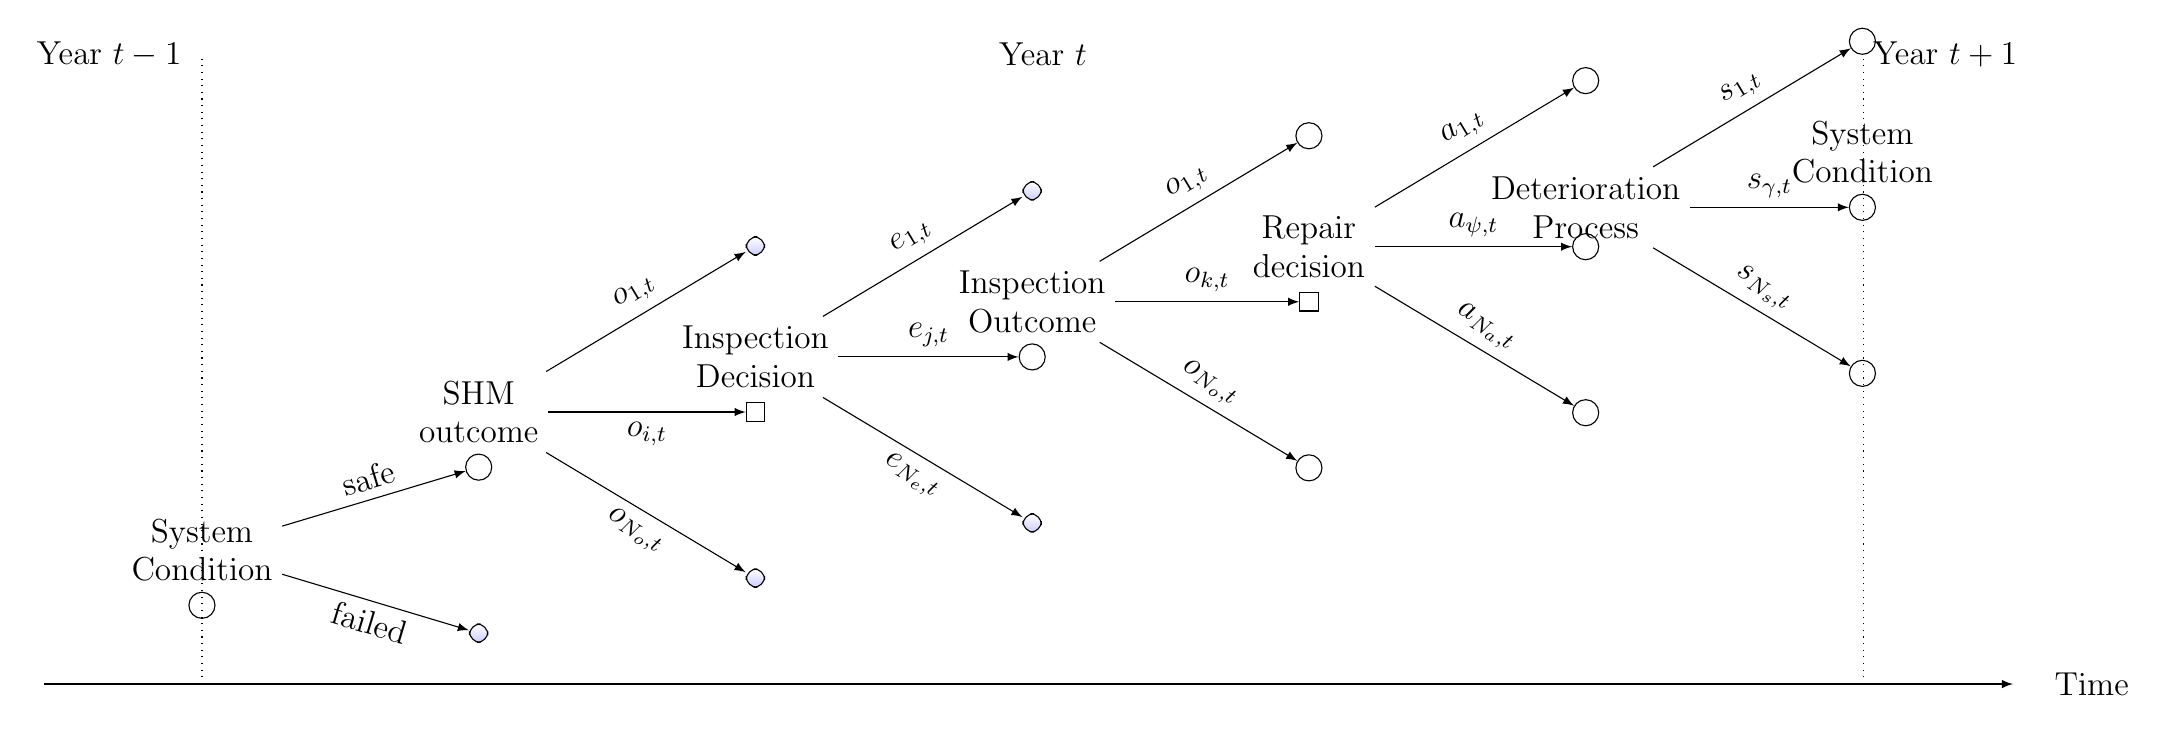
\begin{tikzpicture}
		[
		grow                    = right,
		sibling distance        = 6em,
		level distance          = 10em,
		edge from parent/.style = {draw, -latex},
		every node/.style       = {font=\large},
		sloped
		]
		\node [dummy] {} node [yshift=7mm,align=center]{System \\ Condition}
		child { node [env] {}
			edge from parent node [below] {failed} }
		child { node [dummy] {} node [yshift = 7mm,align=center] {SHM \\ outcome}
			child { node [env] {}
				edge from parent node [below, align=center]
				{$o_{N_o,t}$}}
			child { node [dummy,rectangle] {} node [yshift = 7mm,align = center] {Inspection\\ Decision}
				child { node [env] {}
					edge from parent node [below] {$e_{N_e,t}$} }
				child { node [dummy]{} node[yshift=7mm,align=center] {Inspection\\ Outcome}
					child {node [dummy] {}
						edge from parent node [above] {$o_{N_o,t}$}}
					child {node [dummy,rectangle] {} node[yshift=7mm,align=center]{Repair \\ decision}
						child{node[dummy]{}
							edge from parent node [above]{$a_{N_a,t}$}}
						child{node[dummy]{}node[yshift=5mm, align =center]{Deterioration \\ Process}
							child{node[dummy]{}
								edge from parent node [above]{$s_{N_s,t}$}}
							child{node[dummy]{} node [yshift=7mm, align= center] {System \\ Condition}
								edge from parent node [above]{$s_{\gamma,t}$}}
							child{node[dummy]{}
								edge from parent node [above]{$s_{1,t}$}}
							edge from parent node [above] {$a_{\psi,t}$}}
						child{node[dummy]{}
							edge from parent node [above]{$a_{1,t}$}}
						edge from parent node [above] {$o_{k,t}$}}
					child {node [dummy] {}
						edge from parent node [above] {$o_{1,t}$}}
					edge from parent node [above] {$e_{j,t}$} }
				child { node [env] {}
					edge from parent node [above] {$e_{1,t}$} }
				edge from parent node [below] {$o_{i,t}$} }
			child { node [env] {}
				edge from parent node [above, align=center]
				{$o_{1,t}$}}
			edge from parent node [above] {safe} };
			
	 % draw the time scale line
	 \draw [-latex] (-2,-1) --++(25,0) node [xshift = 10mm] {Time};
	 % 
	 \draw[dotted] (0,-1) --++ (0,8) node [left,align=center] {Year  $t-1$ };% node [right,align=center] {Specific Event happens}; 
	 \node[right] at (10,7)  {Year  $t$};
	 \draw[dotted] (21.1,-1) --++ (0,8) node [right] {Year  $t+1$};
	\end{tikzpicture}
\end{document}